%!TEX root = ../pres.tex
\begin{frame}
\frametitle{The Core Idea}
\begin{center}
  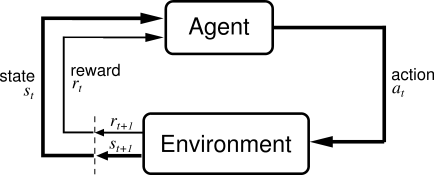
\includegraphics[width=0.5\textwidth]{reinforcementlearning.png}
\end{center}
\begin{itemize}
  \item Models (agents) take action $a_t$ in some environment.
  \item Environment provides state $s_t$, reward $r_t$.
  \item Models learn to maximize reward $r_t$, $\forall t$.
\end{itemize}
\end{frame}




\begin{frame}
  \frametitle{Markov Decision Process (MDP)}
      Environment, $E = (\mathcal{S}, \mathcal{A}, \mathcal{R}, \rho, r)$. 
        \begin{enumerate}
        \item State space, $\mathcal{S}$
        \item Action space, $\mathcal{A}$
        \item Reward space, $\mathcal{R}$   
        \item Transition distribution, $\rho(s'\ |\ s,a)$. Given a previous state $s$ and action $a$, environment gives $s'$.
        \item Reward function $r(s,a) \in \mathcal{R}$.
        \end{enumerate}
        \textbf{Markov Property:} $\rho(s'\ |\ s,a)$ depends only on $s,a$ not previous states!
\end{frame} 

\begin{frame}
  \frametitle{Markov Decision Process (MDP)}
  \begin{center}
  \textbf{Example MDP}
        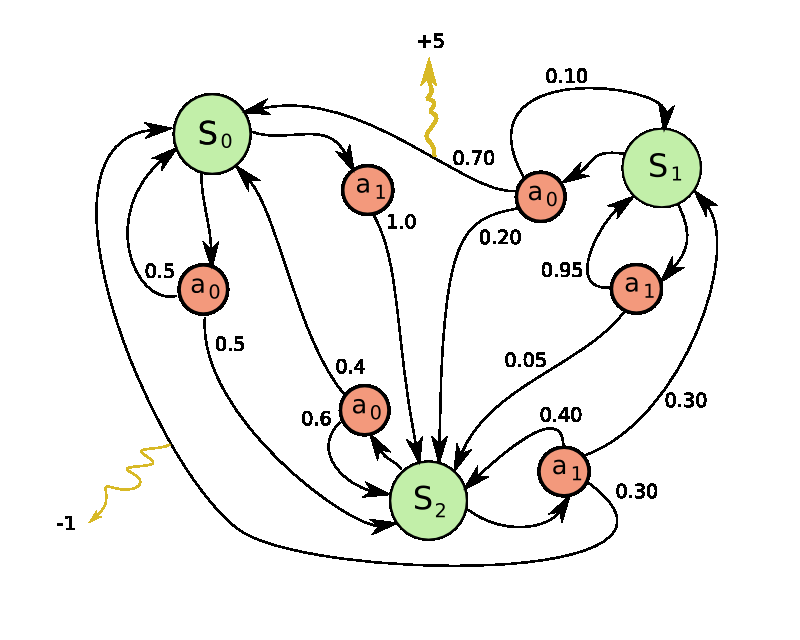
\includegraphics[width=0.9\textwidth]{Markov_Decision_Process_example.png}
  \end{center}
\end{frame}



\begin{frame}
  \frametitle{Pacman as an MDP}
    \begin{columns}
    \begin{column}{0.5\textwidth}
      \begin{itemize}
        \item $\scripts = \mathbb{R}^{256\times 256},$ images as state space.
        \item $\scripta = \{\uparrow, \downarrow, \rightarrow, \leftarrow\}$, joystick as action space.
        \item $r(s_t,a_t) = $ change in score.
        \item $\rho(s_{t+1}\ |\ s_t, a_t) = $ next frame of game after joystick action $a_t$.
      \end{itemize}
    \end{column}
    \begin{column}{0.5\textwidth}
    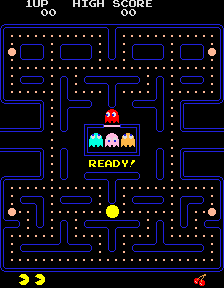
\includegraphics[width=0.9\textwidth]{Pac-man.png}
    \end{column}
  \end{columns}
\end{frame}



\begin{frame}[fragile]
  \frametitle{Policies/Agents}
\textbf{Two different types of agents}
    \begin{itemize}
    \item Deterministic policy $a = \pi(s)$ acts in $E$. 
    \item Stochastic policy $a \sim \pi(a | s)$ gives a probability distibution over actions.
    \end{itemize}

\textbf{Policy Trajectories}
    
    \begin{equation*}
      \begin{tikzcd}
          s_1 \arrow{r}{\pi} & a_1 \arrow{r}{\rho, r} & s_2, r_2 \arrow{r}{\pi}& a_2  \arrow{r}{\rho, r} & \cdots
         \end{tikzcd}   
    \end{equation*}
\end{frame}




\begin{frame}
\frametitle{Value under a policy}
  The \textbf{state value} is a function of a given state for an agent $\pi$ defined as 
  \begin{equation*}
    V^\pi(s_t) = \mathbb{E}\left[\sum_{n={t+1}}^\infty \gamma^n r(s_n, \pi(s_n))\right]
  \end{equation*} 
  \begin{enumerate}
    \item $\gamma$ is the discount factor
    \item $\pi(s_n)$ is the action the agent $\pi$ makes after seeing state $s_n$.
    \item $r(s_n, \pi(s_n))$ is the reward the agent gets from taking that action.
  \end{enumerate}
\end{frame}


\begin{frame}[fragile]
\frametitle{Value under a policy}
  The \textbf{state value} is a function of a given state for an agent $\pi$ defined as 
  \begin{equation*}
    V^\pi(s_t) = \mathbb{E}\left[\sum_{n={t+1}}^\infty \gamma^n r(s_n, \pi(s_n))\right]
  \end{equation*} 
    \begin{equation*}
      \begin{tikzcd}
          s_t \arrow{r}{\pi} & a_1 \arrow{r}{\rho, r} & s_2, r_2 \arrow{r}{\pi}& a_2  \arrow{r}{\rho, r} & \cdots
         \end{tikzcd}    
    \end{equation*}
  \begin{equation*}
        \begin{tikzcd}
        s_t \arrow{r}{\pi} & a_0 \arrow{r}{\rho, r} & s_7, r_7 \arrow{r}{\pi}& a_3  \arrow{r}{\rho, r} & \cdots
       \end{tikzcd} 
  \end{equation*}
\end{frame}



\begin{frame}
\frametitle{Value under a policy}
  The \textbf{state-action value} for an agent $\pi$ is defined such that
  \begin{equation*}
    Q^\pi(s_t, a_t) = \mathbb{E}\left[\underbrace{r(s_t, a_t)}_{\text{reward for } a_t} + V^\pi(s_t)\right]
  \end{equation*}
  \begin{itemize}
    \item Given some state $s_t$, the \emph{best} agent, $\pi^*$ is one that take action 
  \begin{equation*}
    a_t = \argmax_a Q(s_t, a).   
  \end{equation*}
  \end{itemize}
\end{frame}

\begin{frame}
  \frametitle{Problems in Reinforcement Learning}
  \begin{itemize}
    \item \textbf{Policy Optimization:} maximize the expected reward with respect to a policy $\pi$;
    \begin{equation*}
      \pi^* = \argmax_\pi \mathbb{E}\left[\sum_{t=0}^\infty r_t \right]
    \end{equation*}
    \item \textbf{Policy Evaluation:} Given some fixed policy $\pi$ compute expected return.
    \begin{itemize}
      \item Computing $Q^{\pi}$, $V^{\pi}$, and other expectations on policy rollout.
      \item Lets us perform policy optimization!
    \end{itemize}
  \end{itemize}
\end{frame}
